% Author: Izaak Neutelings (May 2021)
% Description:
%   Construct variables with vectors of jet en MET,
%   like the MT2 variable in SUSY searches.
% Inspiration: https://slidetodoc.com/presentation_image/ff8a8e4c690b62727b0cc4ed74967d46/image-7.jpg
\documentclass[border=3pt,tikz]{standalone}
\usepackage{amsmath}
\usepackage{physics}
\usepackage{xcolor}
\usetikzlibrary{calc}
\tikzset{>=latex} % for LaTeX arrow head
\usetikzlibrary{decorations.pathreplacing} % for curly braces

\colorlet{myblue}{blue!70!black}
\colorlet{mydarkblue}{blue!40!black}
\colorlet{mygreen}{green!40!black}
\colorlet{myred}{red!65!black}
\tikzstyle{vector}=[->,very thick,myblue,line cap=round]
\tikzstyle{ptmiss}=[->,dashed,thick,myred,line cap=round]
\tikzstyle{cone}=[thin,blue!50!black,fill opacity=0.8]

\newcommand*{\vv}[1]{\vec{\mkern0mu#1}} % aligned vector arrow
\newcommand{\ptmiss}{\vv{p}_\mathrm{T}^\mathrm{miss}}
\newcommand*{\ptmissX}[1]{\vv{p}_\mathrm{T}^\mathrm{miss,#1}}
\newcommand*{\MTX}[1]{M_\mathrm{T}^{(#1)}}
\newcommand\cone[4]{
  \pgfmathanglebetweenpoints{\pgfpointanchor{#1}{center}}{\pgfpointanchor{#2}{center}}
  \coordinate (tmpR) at ($(#2)+(\pgfmathresult+90:#3)$);
  \coordinate (tmpL) at ($(#2)+(\pgfmathresult-90:#3)$);
  \draw[blue!80!black] (tmpL) -- (#1) -- (tmpR);
  %\draw[red] (#2)++(\pgfmathresult:#4) circle({sqrt(#3^2+#4^2)});
  \draw[blue!80!black,rotate=\pgfmathresult] (#2) ellipse({#4} and {#3});
}

\newcommand\jetcone[4]{
  \pgfmathanglebetweenpoints{\pgfpointanchor{#1}{center}}{\pgfpointanchor{#2}{center}}
  \edef\tmpang{\pgfmathresult}
  \coordinate (tmpO) at ($(#1)+(\tmpang:0.02)$); % center
  \coordinate (tmpC) at ($(#2)+(\tmpang-180:{abs(#4)+0.4})$); % center
  \coordinate (tmpL) at ($(tmpC)+(\tmpang+90:#3)$); % left corner
  \coordinate (tmpR) at ($(tmpC)+(\tmpang-90:#3)$); % right corner
  \draw[thin,blue!50!black,fill opacity=0.8, %,fill=blue!50!black!30
        top color=blue!50!black!50,bottom color=blue!50!black!60,shading angle=\tmpang,rotate=\tmpang]
    %(tmpR) arc(90:-90:{#4} and {#3});
    (tmpC) ellipse({#4} and {#3});
  \begin{scope}
    \clip[rotate=\tmpang] (tmpR) -- (tmpO) -- (tmpL) arc(90:-90:{#4+0.6} and {#3});
    \draw[vector] (tmpO) -- (#2);
  \end{scope}
  \draw[thin,blue!50!black,fill opacity=0.8, %,fill=blue!50!black!30
        top color=blue!50!black!30,bottom color=blue!40!black!50,shading angle=\tmpang,rotate=\tmpang]
    (tmpL) arc(90:270:{#4} and {#3}) -- (tmpO) -- cycle;
}


\begin{document}


% MT2
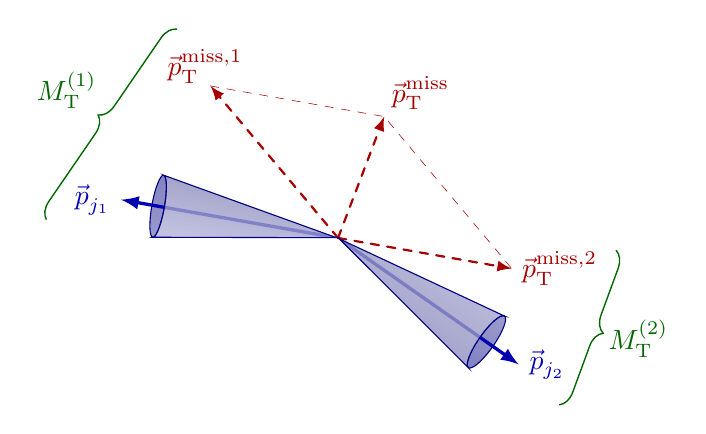
\begin{tikzpicture}
  \def\R{2.8}
  \coordinate (O) at (0,0);
  \coordinate (J1) at (170:\R); % jet 1 pT
  \coordinate (J2) at (-35:\R); % jet 2 pT
  \coordinate (M1) at (130:0.9*\R); % pTmiss component 1
  \coordinate (M2) at (-10:0.8*\R); % pTmiss component 2
  \coordinate (M) at ($(M1)+(M2)$); % total missing momentum
  
  % PTMISS
  \draw[ptmiss,-,very thin] (M1) -- (M) -- (M2);
  \draw[ptmiss] (O) -- (M1) node[left=2,above=-3] {$\ptmissX{1}$};
  \draw[ptmiss] (O) -- (M2) node[right=0] {$\ptmissX{2}$};
  \draw[ptmiss] (O) -- (M) node[above right=-1] {$\ptmiss$};
  
  % JET CONES
  %\draw[vector] (O) -- (J1);
  %\draw[vector] (O) -- (J2);
  %\cone{O}{J1}{0.3}{0.15}
  \jetcone{O}{J1}{0.4}{0.08}
  \jetcone{O}{J2}{0.4}{0.10}
  \node[vector,left] at (J1) {$\vv{p}_{j_1}$};
  \node[vector,right] at (J2) {$\vv{p}_{j_2}$};
  
  % CURLY BRACE
  \draw[line width=0.5,mygreen,decorate,decoration={brace,amplitude=6}]
    ($(J1)+(195:0.35*\R)$) -- ($(M1)+(120:0.30*\R)$) node[midway,above left=2] {$\MTX{1}$};
  \draw[line width=0.5,mygreen,decorate,decoration={brace,amplitude=6}]
    ($(M2)+(10:0.48*\R)$) -- ($(J2)+(-45:0.26*\R)$) node[midway,below=4,right=4] {$\MTX{2}$};
  
\end{tikzpicture}


% MT2 in 3D
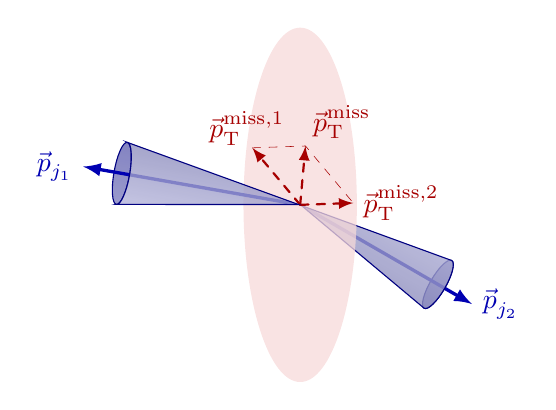
\begin{tikzpicture}
  \def\R{2.8}
  \def\M{0.9}
  \coordinate (O) at (0,0);
  \coordinate (J1) at (170:\R); % jet 1 pT
  \coordinate (J2) at (-30:0.90*\R); % jet 2 pT
  \coordinate (M1) at (130:1.05*\M); % pTmiss component 1
  \coordinate (M2) at (2:0.75*\M); % pTmiss component 2
  \coordinate (M) at ($(M1)+(M2)$); % total missing momentum
  
  % JET CONE BACK
  \jetcone{O}{J2}{0.35}{-0.1}
  \node[vector,right] at (J2) {$\vv{p}_{j_2}$};
  
  % PTMISS
  \fill[red!80!black!15,opacity=0.75] % transverse plane
    (O) ellipse ({0.8*\M} and {2.5*\M});
  \draw[ptmiss,-,very thin] (M1) -- (M) -- (M2);
  \draw[ptmiss] (O) -- (M1) node[left=2,above=-3] {$\ptmissX{1}$};
  \draw[ptmiss] (O) -- (M2) node[right=0] {$\ptmissX{2}$};
  \draw[ptmiss] (O) -- (M) node[above right=-1] {$\ptmiss$};
  
  % JET CONE FRONT
  \jetcone{O}{J1}{0.4}{0.1}
  \node[vector,left] at (J1) {$\vv{p}_{j_1}$};
  
\end{tikzpicture}


\end{document}